\section{Examples}

\subsection{Nomystery}

\subsubsection*{Explanation Domain}
The goal in nomystery is to deliver packages from a initial location (labeled in red)
to a goal location (labeled in green). There are two trucks with a separate fuel level.
The amount of packages a truck can transport is not limited. A truck can either load or 
unload a package or drive from one to an other location. Loading and unloading costs no fuel,
driving costs between 1 and 5 fuels units (label at the edges).\\

Properties:
\begin{itemize}
	\item don't use $T_i$ $(L_x,L_y)$: Truck $T_i$ should not drive from $L_x$ to
		$L_y$ or vise versa
	\item use $T_i$ $(L_x,L_y)$: Truck $T_i$ should drive at least once from $L_x$ to
		$L_y$ or vise versa
	\item same truck $P_x$ $P_y$: both packages have to be delivered by the same truck
		(the packages are either only loaded and an unloaded by truck $T_0$ or by $T_1$)
\end{itemize}

\subsubsection*{Example 1}
%\begin{figure}
	The fuel limit is 1.5 times the minimal limit to deliver all packages.

	Initial fuel:
	$fuel(T_0) = 16$, $fuel(T_1) = 7$

	\begin{center}
	\begin{tikzpicture}
		\node[draw, circle, label=above:{\textcolor{red}{$P_0, P_1,P_2$}}] (l0) at (0,0) {$L_0$};
		\node[draw, circle, label=right:{$T_1$}] (l1) at (4,-1) {$L_1$};
		\node[draw, circle] (l2) at (6,0) {$L_2$};
		\node[draw, circle, label=right:{\textcolor{darkgreen}{$P_1$}}] (l3) at (6,-3) {$L_3$};
		\node[draw, circle, label=below:{\textcolor{darkgreen}{$P_0$}}] (l4) at (2,-2) {$L_4$};
		\node[draw, circle, label=below:{$T_0$ \textcolor{darkgreen}{$P_2$}}] (l5) at (0,-3) {$L_5$};

		\draw[thick] (l0) to node[above] {5} (l2);
		\draw[thick] (l0) to node[above] {2} (l1);
		\draw[thick] (l0) to node[above] {3} (l4);
		\draw[thick] (l0) to node[left] {4} (l5);
		\draw[thick] (l2) to node[right] {1} (l3);
		\draw[thick] (l4) to node[above] {2} (l1);
		\draw[thick] (l4) to node[above] {5} (l3);
		\draw[thick] (l5) to node[below] {5} (l3);
		\draw[thick] (l4) to node[below] {4} (l5);
	\end{tikzpicture}
	\end{center}
	\begin{minipage}[t]{0.3\textwidth}
	Properties:
	\begin{enumerate}
		\item use $T_0$ $(L_2,L_3)$
		\item same truck $P_1$ $P_2$
		\item use $T_0$ $(L_4,L_3)$
		\item same truck $P_2$ $P_0$
		\item don't use $T_0$ $(L_0,L_5)$
		\item use $T_1$ $(L_5,L_4)$
	\end{enumerate}
	\end{minipage}
	\begin{minipage}[t]{0.15\textwidth}
		MUGS:
		\begin{itemize}
			\item $\{4,5,6\}$
			\item $\{2,5,6\}$
			\item $\{3,4,5\}$
			\item $\{3,4,5\}$
			\item $\{2,4,5\}$
			\item $\{2,3,5\}$
			\item $\{1,3,4\}$
			\item $\{1,2,3\}$
		\end{itemize}
	\end{minipage}

\subsection{Blocksworld}

The cost bound is set to 11, 0.5 times the minimal cost to solve all goals.
You can pick up and put down a block from the table and stack and unstack two blocks.
Each of these actions costs 1.

\begin{center}
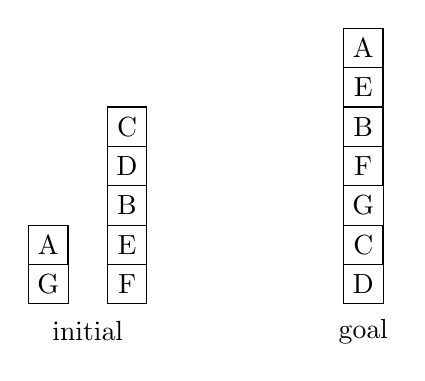
\begin{tikzpicture}
	\node[draw, minimum size=0.5cm] (G) at (0,0) {G};
	\node[draw, minimum size=0.5cm] (A) at (0,0.5) {A};

	\node[draw, minimum size=0.5cm] (F) at (1,0) {F};
	\node[draw, minimum size=0.5cm] (E) at (1,0.5) {E};
	\node[draw, minimum size=0.5cm] (B) at (1,1) {B};
	\node[draw, minimum size=0.5cm] (D) at (1,1.5) {D};
	\node[draw, minimum size=0.5cm] (C) at (1,2) {C};
	\node[] (i) at (0.5,-0.6) {initial};


	\node[draw, minimum size=0.5cm] (D) at (4,0) {D};
	\node[draw, minimum size=0.5cm] (C) at (4,0.5) {C};
	\node[draw, minimum size=0.5cm] (G) at (4,1) {G};
	\node[draw, minimum size=0.5cm] (F) at (4,1.5) {F};
	\node[draw, minimum size=0.5cm] (B) at (4,2) {B};
	\node[draw, minimum size=0.5cm] (E) at (4,2.5) {E};
	\node[draw, minimum size=0.5cm] (A) at (4,3) {A};
	\node[] (g) at (4,-0.6) {goal};
\end{tikzpicture}
\end{center}

MUGS:
\begin{itemize}
	\item $\{on(E,B), on(G,C)\}$
	\item $\{on(A,E), on(C,D), on(G,C)\}$
	\item $\{on(B,F), on(G,C)\}$
	\item $\{on(F,G)\}$
	\item $\{on(A,E), on(C,D), on(E,B)\}$
	\item $\{on(B,F), on(E,B)\}$
	\item $\{on(B,F), on(C,D)\}$
	\item $\{on(A,E), on(B,F)\}$
\end{itemize}


